\documentclass[conference]{IEEEtran}
\IEEEoverridecommandlockouts
\usepackage{cite}
\usepackage{amsmath}
\usepackage{graphicx}
\usepackage[T1]{fontenc}
\usepackage[utf8]{inputenc}
\usepackage{booktabs}
\usepackage{url}
\usepackage[hidelinks]{hyperref}

\begin{document}

\title{Grey Is All Theory: Spatial Aggregation and the Limits of Civic
Evidence in Leipzig's Open Data}

\author{\IEEEauthorblockN{Jonas Paul}
\IEEEauthorblockA{Computational Spatial Humanities\\
Universit\"at Leipzig}
\and
\IEEEauthorblockN{Lucas Berger}
\IEEEauthorblockA{Computational Spatial Humanities\\
Universit\"at Leipzig}}

\maketitle

\begin{abstract}
% 150-200 words, written last.
\end{abstract}

\begin{IEEEkeywords}
open government data, urban dashboards, spatial aggregation, modifiable areal
unit problem, critical data studies
\end{IEEEkeywords}

\begin{flushright}
\itshape
\small
``Denn was man schwarz auf wei\ss{} besitzt, / Kann man getrost nach Hause
tragen.''\footnotemark\\
--- Goethe, \textit{Faust I}, V.~1966 f.
\end{flushright}
\footnotetext{``For what one owns in black and white, one can carry home
with confidence.''}

\section{Introduction}

\section{Background and Related Work}

\section{The Data Landscape and Its Frictions}

\section{System Design}

\begin{figure*}[t]
\centering
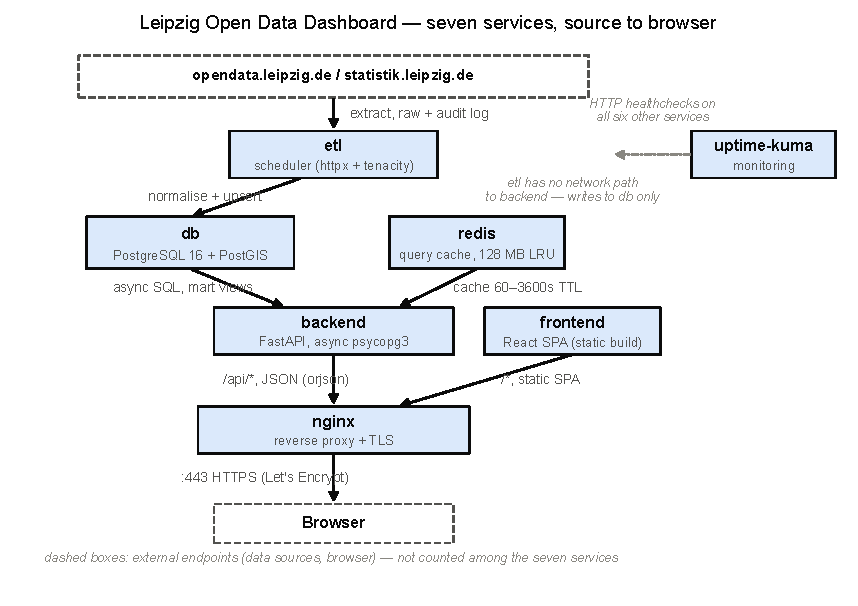
\includegraphics[width=0.85\textwidth]{figures/fig1_architecture.pdf}
\caption{The seven-service architecture of the dashboard and the path a
dataset takes from the open data portal to the browser.}
\label{fig:architecture}
\end{figure*}

\section{Results}

\begin{figure}[t]
\centering
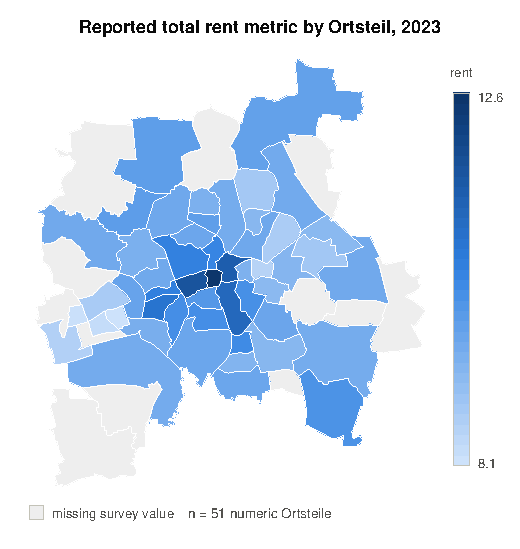
\includegraphics[width=\linewidth]{figures/fig2_choropleth.pdf}
\caption{Voter turnout per Ortsteil in the 2024 European election. Turnout
ranges from 51\% in Gr\"unau-Nord to 83\% in Baalsdorf.}
\label{fig:choropleth}
\end{figure}

\begin{figure}[t]
\centering
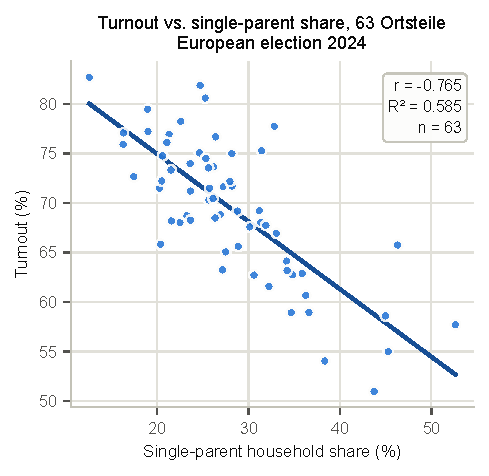
\includegraphics[width=\linewidth]{figures/fig3_scatter.pdf}
\caption{Turnout against the single-parent share of families across 63
Ortsteile ($r = -0.765$, $R^2 = 0.585$).}
\label{fig:scatter}
\end{figure}

\begin{figure*}[t]
\centering
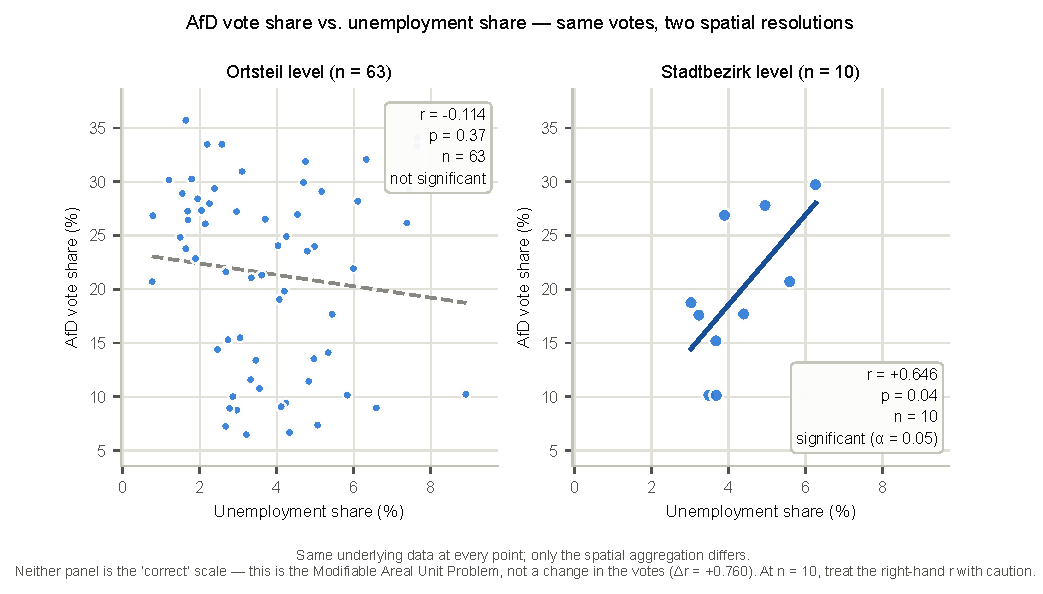
\includegraphics[width=0.85\textwidth]{figures/fig4_maup.pdf}
\caption{AfD vote share against registered unemployment, re-aggregated at
two spatial scales (Ortsteil, $n=63$, vs.\ Stadtbezirk, $n=10$). Neither
scale is the correct one, and the resulting $n=10$ coefficient must not be
read as a finding.}
\label{fig:maup}
\end{figure*}

\section{Discussion: Transparency and Its Infrastructure}

\section{Limitations and Future Work}

\section{Conclusion}

\bibliographystyle{IEEEtran}
% \nocite{*} renders every entry in refs.bib even though none are cited
% in the body yet. The prose task should remove this line once citations
% are added throughout the text.
\nocite{*}
\bibliography{refs}

\end{document}
